\begin{textblock}{\mycolwidth}(\leftpos,2.5)
\LHead{Introduction} \\
\large
Various routing models each considering some aspects of finding ``best''
solutions:
\begin{itemize}
  \item Shortest Path Problem: Finding a shortest path also yields an efficient path regarding energy consumption.
  \item Shortest Weight-Constrained Path Problem: Optimize more than one target function, e.g.\ time and energy-consumption.
  \item Time-Dependent and Multi-Modal Routing: Finding shortest paths depending on the time, caused for example by including public transportation.
  \item Energy-Optimal Routing: Considering energy constraints for electric vehicles.
  \item Stochastic Routing: Minimizing expected costs, maybe given certain conditional probabilities.
  \item Rerouting: After finding an efficient path and turning to a different direction (or gaining additional information),
  quickly find an alternate efficient route.
\end{itemize}
Each model comes with its own set of algorithms,
our aim is to find a model unifying some aspects while still
allowing for most algorithms known for the shortest path problem.
\end{textblock}

\begin{textblock}{\mycolwidth}(\leftpos,10)
\LHead{Functional Routing}\\
\large
\begin{center}
\begin{tikzpicture}[scale=2.8]
  \node[vertex] (v0) at (0, 4.7) {$v_0$};
  \node[vertex] (v1) at (2.5, 4.95) {$v_1$};
  \node[vertex] (v2) at (5, 4.45) {$v_2$};
  \node[vertex] (v3) at (7.5, 4.7) {$v_3$};
  \path[edge] (v0) -- (v1);
  \path[edge] (v1) -- (v2);
  \path[edge] (v2) -- (v3);
  \node[draw,minimum height=5.7cm,minimum width=1.6cm] at (0,2) {};
  \node[draw,minimum height=5.7cm,minimum width=1.6cm] at (2.5,2) {};
  \node[draw,minimum height=5.7cm,minimum width=1.6cm] at (5,2) {};
  \node[draw,minimum height=5.7cm,minimum width=1.6cm] at (7.5,2) {};
  \node[circle] (s) at (0, 1.5) {$s_0$};
  \node[circle] (ss) at (2.5, 1.7) {$s_1$};
  \node[circle] (sss) at (5, 2.2) {$s_2$};
  \node[circle] (ssss) at (7.5, 2.4) {$s_3$};
  \path[edge] (s) -- (ss);
  \path[edge] (ss) -- (sss);
  \path[edge] (sss) -- (ssss);
  \node[align=center] (edgelabels) at (-1.7,3.75) {labels are functions};
  \node[align=center] (init) at (-1.5,2) {initial\\ state};
  \path[edge, dashed] (init) -- (s);
  \node[align=center] (final) at (9,2) {final\\ state};
  \path[edge, dashed] (final) -- (ssss);
  \node[align=center] (start) at (-1.5,4.7) {start};
  \path[edge, dashed] (start) -- (v0);
  \node[align=center] (end) at (9,4.7) {end};
  \path[edge, dashed] (end) -- (v3);
  \node (w1) at (1.25, 3.7) {$W(v_0, v_1)$};
  \node (w2) at (3.75, 3.7) {$W(v_1, v_2)$};
  \node (w3) at (6.25, 3.7) {$W(v_2, v_3)$};
  \path[edge, dashed] (1.25,4.5) -- (w1) -- (1.25, 1.8);
  \path[edge, dashed] (3.75,4.3) -- (w2) -- (3.75, 2.1);
  \path[edge, dashed] (6.25,4.2) -- (w3) -- (6.25, 2.5);
\end{tikzpicture}
\end{center}
\end{textblock}

\begin{textblock}{\mycolwidth}(\leftpos,13.7)
\LHead{Prototype} \\
\large
The Technische Universit\"at M\"unchen (TUM) initiated a prototypic routing service,
which is further developed at the University of L\"ubeck,
available at \url{www.isp.uni-luebeck.de/greennav}. It is used
to provide and evaluate different routing algorithms. The polygon shows the range prediction of an electric vehicle.
\begin{center}
\resizebox{5\TPHorizModule}{!}{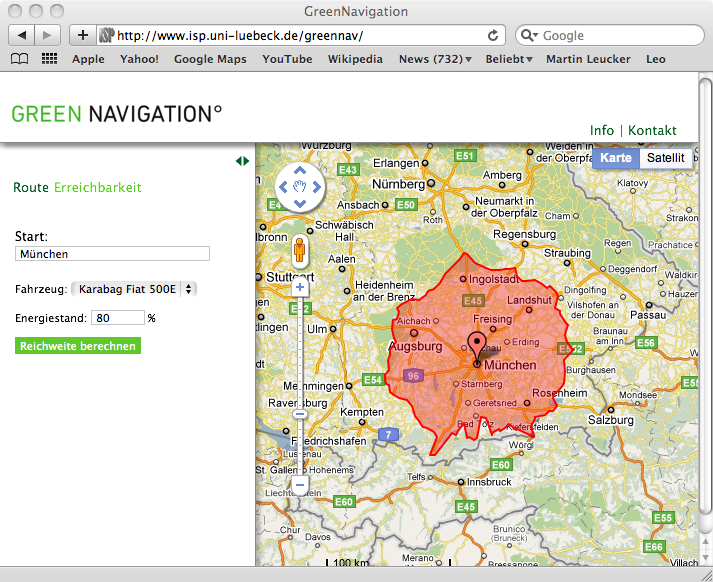
\includegraphics{greennav.png}}
\end{center}
\end{textblock}
